\section{WOMBAT Setup for Eclipse}
To fetch the released code from SVN, make a checkout to \url{https://sw6-2012.googlecode.com/svn/tags/wombat/}, previous versions of the project, reports, and the wiki can be found by making a checkout to \url{https://sw6-2012.googlecode.com/svn/}.
The folders on SVN contains the following:

	\begin{itemize}
		\item \textit{trunk} - contains iteration releases of the code.
		\item \textit{branches} - contains code under development.
		\item \textit{tags} - contains the newest final release of the code.
		\item \textit{common\_report} - contains the common part of the report.
		\item \textit{Reports} - contains all group reports.
		\item \textit{wiki} - contains summaries from all group- and supervisor meetings, and guides/agreements.
	\end{itemize}
	
When SVN checkout has finished downloading content from the SVN, import Wombat, AmbilWarna (the color picker), and wheel projects from svn to Eclipse, figure \ref{fig:import1}.

\begin{figure}[H]
	\centering
		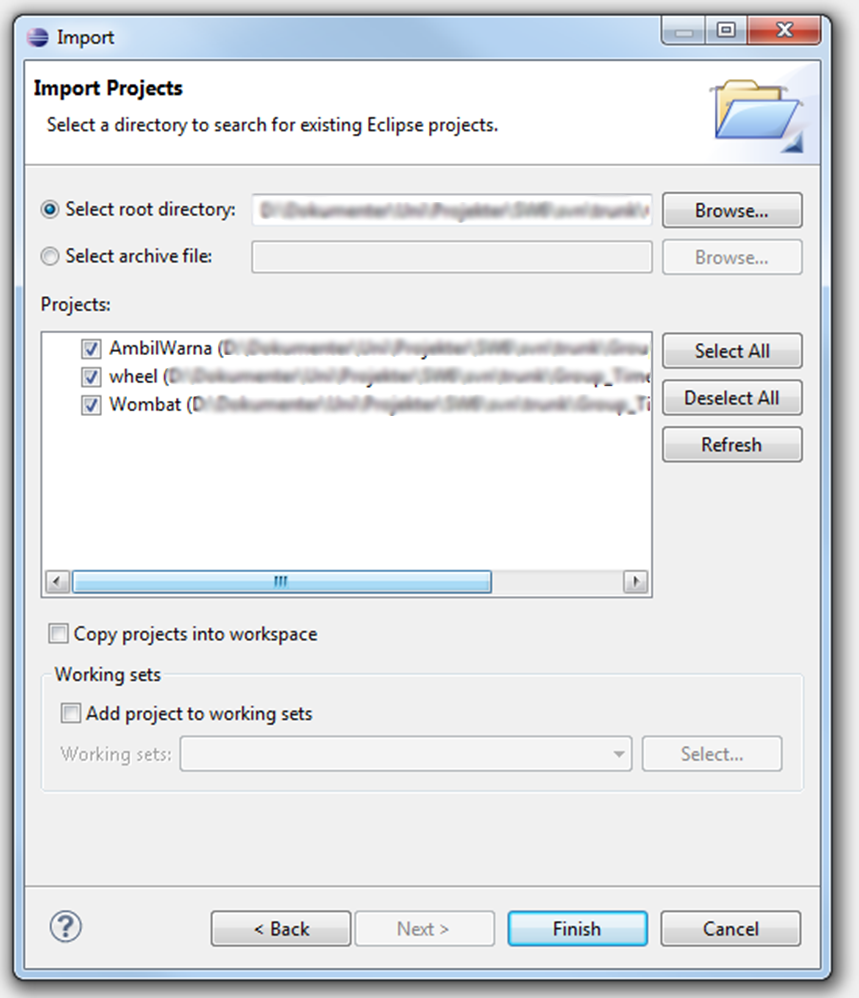
\includegraphics[scale=0.2]{Images/how_to_wombat/import1.png}
	\caption{Import Wombat, AmbilWarna, and wheel.}
	\label{fig:import1}
\end{figure}

Right click the Wombat project in Eclipse and click "Properties".\\
Under the "Android" pane, ensure that AmbilWarna and wheel are added as project libraries, figure \ref{fig:add_libs}.

\begin{figure}[H]
	\centering
		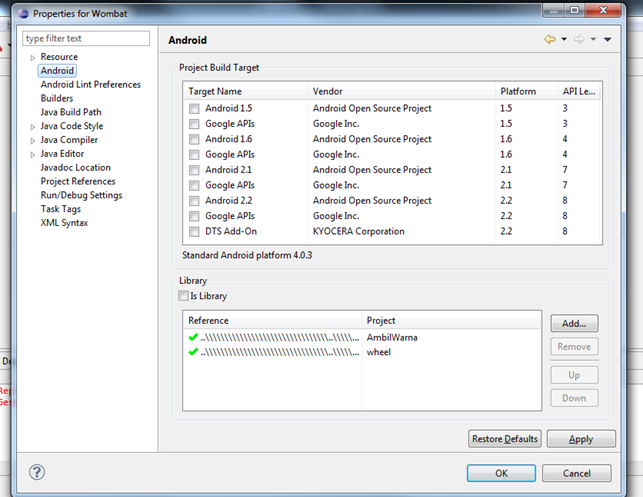
\includegraphics[scale=0.5]{Images/how_to_wombat/add_libs.png}
	\caption{Add AmbilWarna and wheel as project libraries.}
	\label{fig:add_libs}
\end{figure}

In case Eclipse fails to recognize the libraries in the libs folder, manually add the three JAR files in Wombat/libs on svn as external JARs, in Wombat - Properties, figure \ref{fig:external_jar}.

\begin{figure}[H]
	\centering
		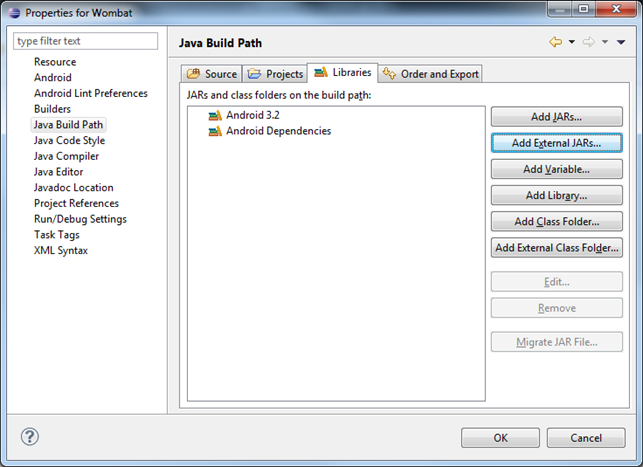
\includegraphics[scale=0.5]{Images/how_to_wombat/external_jar.png}
	\caption{Add Oasis, \texttt{TimerLib}, and \texttt{DrawLib} as external JARs if Eclipse cant recognize them in the libs folder.}
	\label{fig:external_jar}
\end{figure}

\subsection*{Extras}
To edit the \texttt{TimerLib} and \texttt{DrawLib} the two projects has to be imported to the workspace in Eclipse, figure \ref{fig:import2}.

\begin{figure}[H]
	\centering
		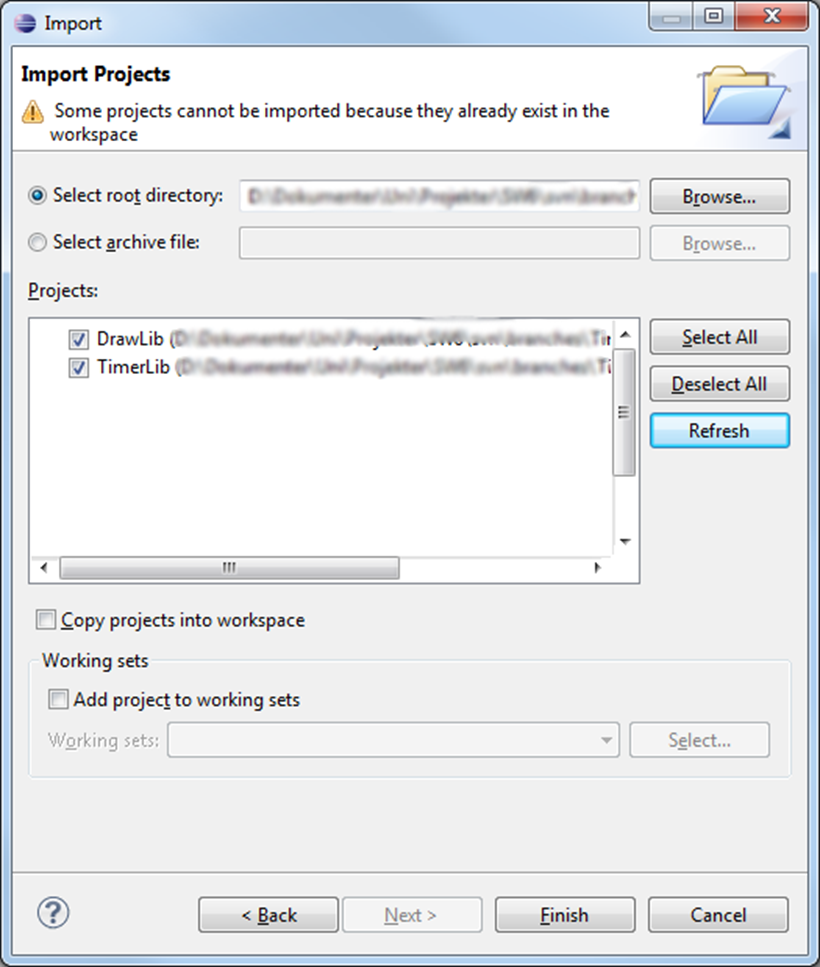
\includegraphics[scale=0.22]{Images/how_to_wombat/import2.png}
	\caption{Import TimerLib and DrawLib to the workspace.}
	\label{fig:import2}
\end{figure}

To debug the \texttt{TimerLib} and \texttt{DrawLib} in WOMBAT the projects has to be added as libraries in the Wombat properties, with AmbilWarna and wheel, figure \ref{fig:add_timer_draw_lib}.
Then the \texttt{TimerLib} and \texttt{DrawLib} JARs has to be deleted from the libs folder or the Java Build Path library, to avoid a compile error.

\begin{figure}[H]
	\centering
		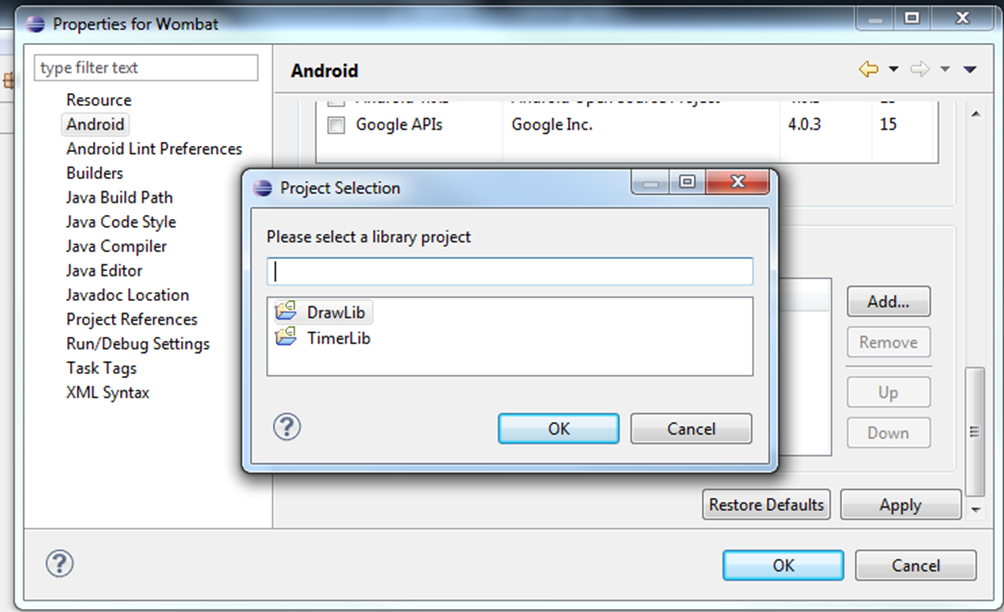
\includegraphics[scale=0.2]{Images/how_to_wombat/add_timer_draw_lib.png}
	\caption{Add \texttt{TimerLib} and \texttt{DrawLib} as project libraries.}
	\label{fig:add_timer_draw_lib}
\end{figure}

\clearpage
\section{GIRAF Installation for Android 3.2 Tablet}
\begin{enumerate}
	\item Find the "How to install" folder
	\item Connect the device to the computer
	\item	Move the two folders Pictogram and GIRAF to the root of the device
	\item	Disconnect the device from the computer.
	\item On the device open the file explorer - e.g. "Mine fil." application
	\item	On the device navigate to the "GIRAF Installer" folder and install the APK file
  \item Click "Installer" and accept all five applications
	\item On the device open OasisApp to insert Test Data - With "Tilføj Test Data"
\end{enumerate}